\documentclass[a4paper,twocolumn]{article}
\usepackage[utf8]{inputenc}
\usepackage{graphicx}
\usepackage{indentfirst}
\usepackage{float}
\usepackage{fancyhdr}
\usepackage{amssymb}
\usepackage{amsmath}
\usepackage{verbatim}
\usepackage{pgfplots}
\usepackage{subcaption}
\usepackage[labelfont=bf]{caption}
\usepackage[top=2.5cm,left=1.5cm,right=1.5cm,bottom=3cm]{geometry}
\newcommand{\HRule}{\rule{\linewidth}{0.5mm}}



\begin{document}
\twocolumn[\begin{@twocolumnfalse}

\begin{center}
\large\textbf{Methods for Feature Extraction on Tiny Images for \textit{k}-Nearest Neighbors Classifiers}
\end{center}

\begin{center}
\small{Eric Miller, University of Georgia at Oxford}\\
\end{center}

\begin{center}
\small{27 June 2020}
\end{center}

\HRule \\
This will be the abstract.    \\
\HRule
\vspace{1cm}

\end{@twocolumnfalse}]

\section{Introduction}
	
    
\section{Methods}
\subsection{\textit{k}-Nearest Neighbors Model}
The \textit{k}-nearest neighbors model was implemented as a Python class, with a methods for training and testing. The \texttt{train} method simply stores the training data, while the \texttt{test} method does the brunt of the work. When the test data is loaded in, L1 distances are computed for every pair of members between the testing and training sets. The \texttt{cdist} function, which uses C-level code, from \texttt{scipy} was used in order to optimize this process.

Next, for each member of the test set, distances to training data members are sorted increasing order, and training labels are sorted accordingly. Hence, the first \textit k training labels in the sorted set can be used to vote for a label for the test data member. For simplicity and speed, \textit k may be passed into the \texttt{test} method, and distances are not recalculated or resorted if not necessary.

A separate model, which interfaced with \texttt{sklearn}'s \texttt{NearestNeighbors} module, was implemented in order to provide a baseline for runtime.

\subsection{Feature extraction}
Originally, the images were fed in as raw pixel values. However, due to the sheer size of the dataset (3072 values for each image), as well as the nature of the model, which would compare the images pixel-by-pixel and not account for invariances, feature extraction methods provided notable increases in testing accuracy. These methods transformed the image arrays into various feature arrays, upon which the model would work and calculate distances.

\subsubsection{Grayscale and Average-Value Images}
The first feature extraction method was a simple grayscale converter. As human vision has different sensitivities to different colors, those with higher sensitivity have greater weight on the grayscale image. For this purpose, the brightness value was the dot product between the RGB array (consisting of 3 floating point values between 0 and 1) and the array \texttt{[0.2989, 0.5870, 0.1140]}.

Average-value images were also created, weighing each original color equally. Both of these methods shrank the 3072-value arrays down to 1024 values. However, they were still subject to the same constraints of \textit k-NN models.

\subsubsection{Spacial Histograms}
One way to combat this issue is to create spacial histograms of pixel values. Within each specified window (e.g., the entire image, quadrants, sixteenths, etc.), and for each color (red, green, and blue), a histogram was calculated for the distribution of the color's brightness across all pixels in the window.

The variable parameters here are window size as well as bin size for the histograms. As window size and bin size increase indefinitely, the spacial histogram gets closer to the raw image, represented in a different (more verbose) format.

Theoretically, this fixes the earlier problem of using raw images (to an extent): instead of comparing raw pixels to pixels in the same locations, distributions of pixel values for each color are compared across general regions.

\subsubsection{Histogram of Oriented Gradients}
In image processing and computer vision, discrete derivatives/gradients are often used for edge detection. Large gradients indicate a strong linear shift in lighting, often indicating the presence of an edge or other feature. A Histogram of Oriented Gradeints (HoG) is a common way of storing the distribution of gradient vectors throughout an image.

The first step to this is determining a grid size, which was fixed at \(8\times8\) pixel squares (forming a \(4\times4\) grid). Within each square, the gradient is calculated for each pixel. The direction derivative is defined as \[D_{\vec{u}}f(\vec{x})\lim_{h\to 0}\frac{f(\vec{x}+h\vec{u})-f(\vec{x})}{h}.\] For \(\vec{u}=\hat{\textbf \i}\), the directional derivative (also the partial derivative with respect to \(x\)) can be discretized as \((f((x,y)+(2,0))-f(x,y))/2\) with \(h=2\) (the smallest distance that avoids half-steps when centering). If we ingore the scale by half (since we care only about directions and relative magnitudes of the gradient), and shift by one, we get the partial derivative \(f_x\approx f(x+1,y)-f(x-1,y)\), which can be represented by the convolution given by kernel \([-1\;0\;1]\). Similarly, for the \(y\) partial, the kernel \([-1\;0\;1]^\top\) may be used.

These convolutions are applied across the images (with 0-padded edges to retain shape) in order to obtain \(8\times8\) matrices of the \(x\) and \(y\) gradients. These are converted to polar coordinates, producing a magnitude and direction for the gradient centered at each of the 64 pixels. Either signed gradients (between -180 and 180) or unsigned gradients (modding by 180, so opposite gradients are represented the same) may be used. This is done for each color, and, for each pixel, the polar tuple with the largest magnitude is used. A histogram is then computed for the directions throughout the square, weighted by their respective magnitudes.

Once each square in the grid is assigned a histogram, they are normalized in groups. Each adjacent \(2\times2\) block of these squares (consisting of \(16\times16\) pixels) is normalized. In a \(32\times32\) resolution image (with a \(4\times4\) grid) there are \(3\times3=9\) possible placements for the normalization block. Within each block, the four histograms are concatenated and normalized (with an L2 norm) in order to account for differences in lighting. All of the normalized histograms are hence concatenated into a single array.

\subsection{Concatenating Multiple Features}
[Will fill in later]

\section{Results and Analysis}

\subsection{\textit k-NN Model}
The custom \textit k-NN completed training and testing for the entire dataset in a total of 2033 seconds, compared to 1984 seconds for the \texttt{sklearn} version.

%knn_no_extract
\begin{figure}[h]
    \centering
    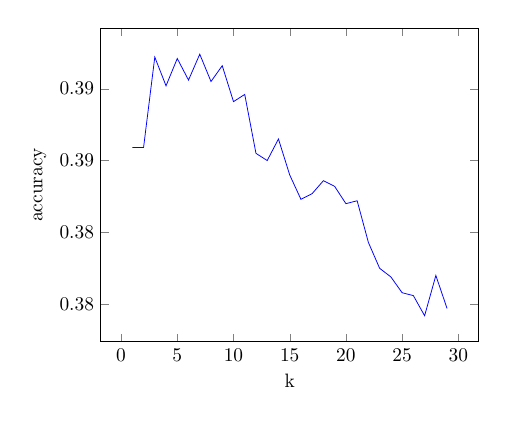
\begin{tikzpicture}[scale=.7]
        \begin{axis}[
            xlabel=k,
            ylabel=accuracy
        ]
        \addplot+[
            mark=none,
        ] plot coordinates{
            (1,0.3859)
            (2,0.3859)
            (3,0.3922)
            (4,0.3902)
            (5,0.3921)
            (6,0.3906)
            (7,0.3924)
            (8,0.3905)
            (9,0.3916)
            (10,0.3891)
            (11,0.3896)
            (12,0.3855)
            (13,0.385)
            (14,0.3865)
            (15,0.384)
            (16,0.3823)
            (17,0.3827)
            (18,0.3836)
            (19,0.3832)
            (20,0.382)
            (21,0.3822)
            (22,0.3793)
            (23,0.3775)
            (24,0.3769)
            (25,0.3758)
            (26,0.3756)
            (27,0.3742)
            (28,0.377)
            (29,0.3747)
        };
        \end{axis}
    \end{tikzpicture}
    \caption{Accuracy of \textit k-NN with raw pixel values.}
    \label{knn_no_extract}
\end{figure}

In figure \ref{knn_no_extract}, we see that

\subsection{Feature Extraction}

\subsubsection{Grayscale and Average-Value}

The image below shows

%knn_grayscale
\begin{figure}[h]
    \centering
    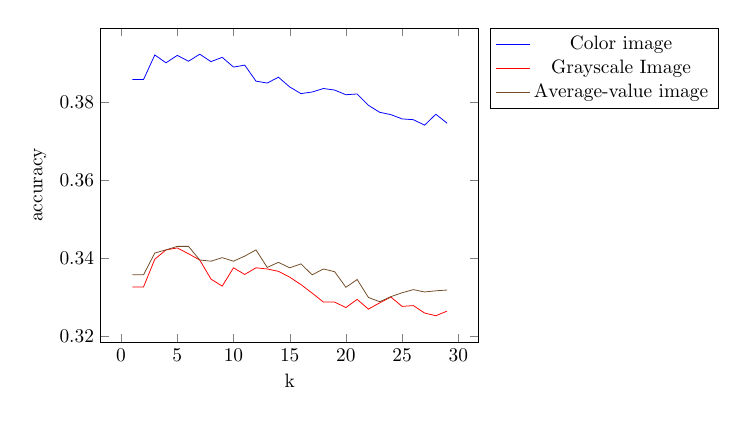
\begin{tikzpicture}[scale=.7]
        \begin{axis}[
            xlabel=k,
            ylabel=accuracy,
            legend pos=outer north east
        ]
        \addplot+[
            mark=none,
        ] plot coordinates{
            (1,0.3859)
            (2,0.3859)
            (3,0.3922)
            (4,0.3902)
            (5,0.3921)
            (6,0.3906)
            (7,0.3924)
            (8,0.3905)
            (9,0.3916)
            (10,0.3891)
            (11,0.3896)
            (12,0.3855)
            (13,0.385)
            (14,0.3865)
            (15,0.384)
            (16,0.3823)
            (17,0.3827)
            (18,0.3836)
            (19,0.3832)
            (20,0.382)
            (21,0.3822)
            (22,0.3793)
            (23,0.3775)
            (24,0.3769)
            (25,0.3758)
            (26,0.3756)
            (27,0.3742)
            (28,0.377)
            (29,0.3747)
        };
        \addlegendentry{Color image}
        \addplot+[
            mark=none,
        ] plot coordinates{
            (1,0.3327)
            (2,0.3327)
            (3,0.3398)
            (4,0.3422)
            (5,0.3427)
            (6,0.3412)
            (7,0.3396)
            (8,0.3347)
            (9,0.3329)
            (10,0.3376)
            (11,0.3359)
            (12,0.3376)
            (13,0.3373)
            (14,0.3367)
            (15,0.3352)
            (16,0.3333)
            (17,0.3311)
            (18,0.3288)
            (19,0.3288)
            (20,0.3274)
            (21,0.3295)
            (22,0.327)
            (23,0.3286)
            (24,0.3301)
            (25,0.3277)
            (26,0.3279)
            (27,0.326)
            (28,0.3253)
            (29,0.3265)
        };
        \addlegendentry{Grayscale Image}
        \addplot+[
            mark=none
        ] plot coordinates {
            (1,0.3358)
            (2,0.3358)
            (3,0.3414)
            (4,0.3422)
            (5,0.3431)
            (6,0.3431)
            (7,0.3396)
            (8,0.3393)
            (9,0.3402)
            (10,0.3393)
            (11,0.3406)
            (12,0.3422)
            (13,0.3377)
            (14,0.339)
            (15,0.3376)
            (16,0.3386)
            (17,0.3358)
            (18,0.3373)
            (19,0.3366)
            (20,0.3326)
            (21,0.3346)
            (22,0.33)
            (23,0.3289)
            (24,0.3302)
            (25,0.3312)
            (26,0.332)
            (27,0.3314)
            (28,0.3317)
            (29,0.3319)
        };
        \addlegendentry{Average-value image}
        \end{axis}
    \end{tikzpicture}
    \caption{Accuracy on color versus grayscale and average-value images.}
    \label{knn_grayscale}
\end{figure}

\subsubsection{Spacial Histograms}

The image below shows

%knn_hist
\begin{figure}[h]
    \centering
    \begin{subfigure}{0.5\textwidth}
        \centering
        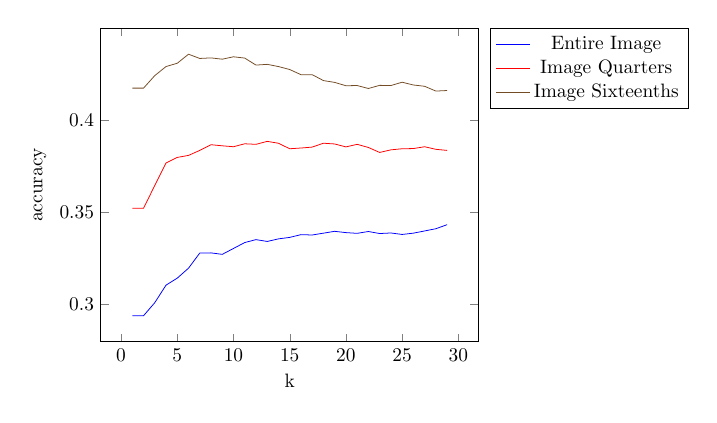
\begin{tikzpicture}[scale=.7]
            \begin{axis}[
                xlabel=k,
                ylabel=accuracy,
                legend pos=outer north east
            ]
            \addplot+[
                mark=none,
            ] plot coordinates{
                (1,0.2937)
                (2,0.2937)
                (3,0.3008)
                (4,0.3103)
                (5,0.3141)
                (6,0.3195)
                (7,0.3277)
                (8,0.3278)
                (9,0.327)
                (10,0.3302)
                (11,0.3334)
                (12,0.335)
                (13,0.334)
                (14,0.3354)
                (15,0.3362)
                (16,0.3377)
                (17,0.3375)
                (18,0.3385)
                (19,0.3395)
                (20,0.3388)
                (21,0.3384)
                (22,0.3394)
                (23,0.3383)
                (24,0.3386)
                (25,0.3378)
                (26,0.3385)
                (27,0.3397)
                (28,0.3409)
                (29,0.3431)
            };
            \addlegendentry{Entire Image};
            \addplot+[
                mark=none,
            ] plot coordinates{
                (1,0.352)
                (2,0.352)
                (3,0.3644)
                (4,0.3766)
                (5,0.3796)
                (6,0.3807)
                (7,0.3834)
                (8,0.3865)
                (9,0.3859)
                (10,0.3854)
                (11,0.387)
                (12,0.3867)
                (13,0.3883)
                (14,0.3873)
                (15,0.3843)
                (16,0.3847)
                (17,0.3852)
                (18,0.3873)
                (19,0.3869)
                (20,0.3853)
                (21,0.3867)
                (22,0.385)
                (23,0.3823)
                (24,0.3837)
                (25,0.3843)
                (26,0.3844)
                (27,0.3854)
                (28,0.384)
                (29,0.3834)
            };
            \addlegendentry{Image Quarters};
            \addplot+[
                mark=none,
            ] plot coordinates{
                (1,0.4172)
                (2,0.4172)
                (3,0.424)
                (4,0.4289)
                (5,0.4307)
                (6,0.4356)
                (7,0.4333)
                (8,0.4336)
                (9,0.4329)
                (10,0.4342)
                (11,0.4335)
                (12,0.4297)
                (13,0.4301)
                (14,0.4289)
                (15,0.4273)
                (16,0.4245)
                (17,0.4245)
                (18,0.4213)
                (19,0.4203)
                (20,0.4185)
                (21,0.4186)
                (22,0.417)
                (23,0.4187)
                (24,0.4186)
                (25,0.4204)
                (26,0.4189)
                (27,0.4182)
                (28,0.4156)
                (29,0.4159)
            };
            \addlegendentry{Image Sixteenths};
            \end{axis}
        \end{tikzpicture}
        \caption{Fixed bin size of 16, with varying window size.\\~\\~\\}
    \end{subfigure}

    \begin{subfigure}{0.5\textwidth}
        \centering
        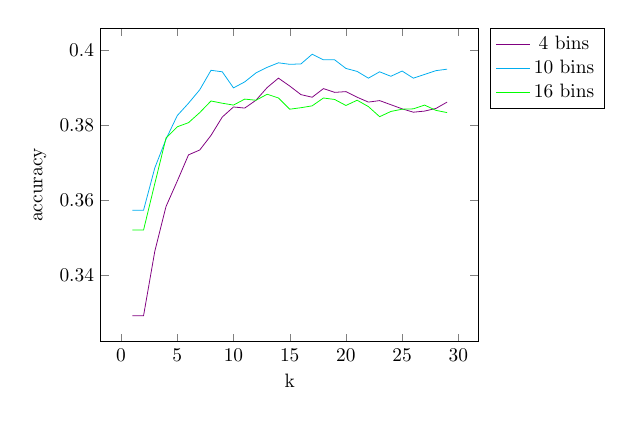
\begin{tikzpicture}[scale=.7]
            \begin{axis}[
                xlabel=k,
                ylabel=accuracy,
                legend pos=outer north east
            ]
            \addplot+[
                mark=none,
                color=violet
            ] plot coordinates{
                (1,0.3291)
                (2,0.3291)
                (3,0.3463)
                (4,0.3583)
                (5,0.3651)
                (6,0.3721)
                (7,0.3734)
                (8,0.3773)
                (9,0.3822)
                (10,0.3849)
                (11,0.3846)
                (12,0.3867)
                (13,0.3901)
                (14,0.3926)
                (15,0.3905)
                (16,0.3882)
                (17,0.3875)
                (18,0.3898)
                (19,0.3888)
                (20,0.389)
                (21,0.3875)
                (22,0.3862)
                (23,0.3866)
                (24,0.3855)
                (25,0.3844)
                (26,0.3835)
                (27,0.3838)
                (28,0.3845)
                (29,0.3862)
            };
            \addlegendentry{4 bins}
            \addplot+[
                mark=none,
                color=cyan
            ] plot coordinates{
                (1,0.3573)
                (2,0.3573)
                (3,0.3686)
                (4,0.3763)
                (5,0.3826)
                (6,0.3859)
                (7,0.3895)
                (8,0.3947)
                (9,0.3943)
                (10,0.39)
                (11,0.3916)
                (12,0.394)
                (13,0.3955)
                (14,0.3967)
                (15,0.3963)
                (16,0.3964)
                (17,0.399)
                (18,0.3975)
                (19,0.3975)
                (20,0.3952)
                (21,0.3944)
                (22,0.3926)
                (23,0.3943)
                (24,0.3931)
                (25,0.3945)
                (26,0.3926)
                (27,0.3936)
                (28,0.3946)
                (29,0.395)
            };
            \addlegendentry{10 bins}
            \addplot+[
                mark=none,
                color=green
            ] plot coordinates{
                (1,0.352)
                (2,0.352)
                (3,0.3644)
                (4,0.3766)
                (5,0.3796)
                (6,0.3807)
                (7,0.3834)
                (8,0.3865)
                (9,0.3859)
                (10,0.3854)
                (11,0.387)
                (12,0.3867)
                (13,0.3883)
                (14,0.3873)
                (15,0.3843)
                (16,0.3847)
                (17,0.3852)
                (18,0.3873)
                (19,0.3869)
                (20,0.3853)
                (21,0.3867)
                (22,0.385)
                (23,0.3823)
                (24,0.3837)
                (25,0.3843)
                (26,0.3844)
                (27,0.3854)
                (28,0.384)
                (29,0.3834)
            };
            \addlegendentry{16 bins}
            \end{axis}
        \end{tikzpicture}
        \caption{Varying bin size, with fixed window size (image quarters).}
    \end{subfigure}
    \caption{Spatial histogram feature extraction results.}
    \label{knn_hist}
\end{figure}

\subsubsection{Histogram of Oriented Gradients}

The following graph reveals

%knn_hog
\begin{figure}[h]
    \centering
    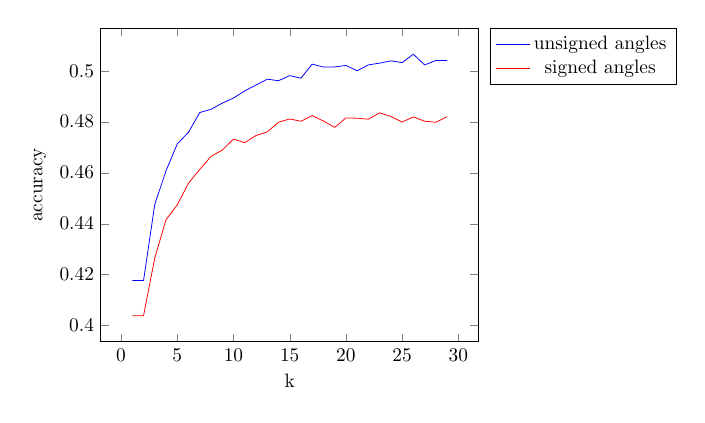
\begin{tikzpicture}[scale=.7]
        \begin{axis}[
            xlabel=k,
            ylabel=accuracy,
            legend pos=outer north east
        ]
        \addplot+[
            mark=none,
        ] plot coordinates{
            (1,0.4177)
            (2,0.4177)
            (3,0.4476)
            (4,0.4608)
            (5,0.4713)
            (6,0.4759)
            (7,0.4836)
            (8,0.4849)
            (9,0.4873)
            (10,0.4893)
            (11,0.4921)
            (12,0.4944)
            (13,0.4967)
            (14,0.4961)
            (15,0.4981)
            (16,0.4971)
            (17,0.5026)
            (18,0.5015)
            (19,0.5015)
            (20,0.5021)
            (21,0.5)
            (22,0.5023)
            (23,0.503)
            (24,0.5039)
            (25,0.5032)
            (26,0.5065)
            (27,0.5023)
            (28,0.504)
            (29,0.504)
        };
        \addlegendentry{unsigned angles}
        \addplot+[
            mark=none,
        ] plot coordinates{
            (1,0.4039)
            (2,0.4039)
            (3,0.4266)
            (4,0.4416)
            (5,0.4474)
            (6,0.4559)
            (7,0.4613)
            (8,0.4664)
            (9,0.4689)
            (10,0.4732)
            (11,0.4718)
            (12,0.4746)
            (13,0.476)
            (14,0.4798)
            (15,0.4811)
            (16,0.4802)
            (17,0.4824)
            (18,0.4803)
            (19,0.4778)
            (20,0.4815)
            (21,0.4814)
            (22,0.481)
            (23,0.4835)
            (24,0.4821)
            (25,0.4799)
            (26,0.4819)
            (27,0.4802)
            (28,0.4798)
            (29,0.482)
        };
        \addlegendentry{signed angles}
        \end{axis}
    \end{tikzpicture}
    \caption{Histogram of Oriented Gradients Extraction.}
    \label{knn_hog}
\end{figure}

\subsection{Concatenation of Multiple Features}

The first graph

%knn_concat_steps
\begin{figure}[H]
    \centering
    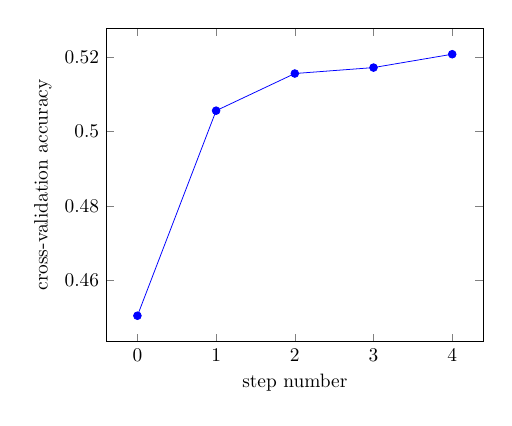
\begin{tikzpicture}[scale=.7]
        \begin{axis}[
            xlabel=step number,
            ylabel=cross-validation accuracy
        ]
        \addplot[
            color=blue,
            mark=*
        ] plot coordinates{
            (0, 0.4504)
            (1, 0.5056)
            (2, 0.5156)
            (3, 0.5172)
            (4, 0.5208)
        };
        \end{axis}
    \end{tikzpicture}
    \caption{Steps of hill climbing search for concatenation weights.}
    \label{knn_concat_steps}
\end{figure}

The second graph

%knn_bar
\begin{figure}[H]
    \centering
    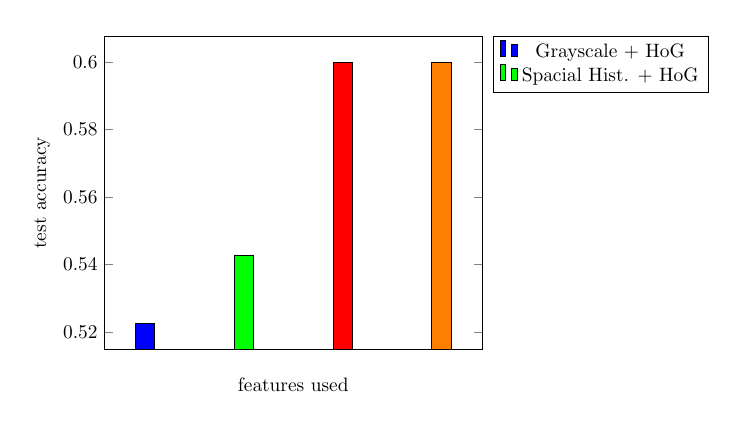
\begin{tikzpicture}[scale=.7]
        \begin{axis}[
            legend pos=outer north east,
            ylabel=test accuracy,
            xlabel=features used,
            xmin=0,
            xmax=5,
            ybar,
            xtick style={draw=none},
            xticklabels={,,,}
        ]
        \addplot[
            fill=blue
        ] plot coordinates{
            (1, 0.5225)
        };
        \addlegendentry{Grayscale + HoG}
        \addplot[
            fill=green
        ] plot coordinates{
            (2, 0.5428)
        };
        \addlegendentry{Spacial Hist. + HoG}
        \addplot[
            fill=red
        ] plot coordinates{
            (3, 0.6) %unknown
        };
        \addplot[
            fill=orange
        ] plot coordinates{
            (4, 0.6) %unknown
        };
        \end{axis}
    \end{tikzpicture}
    \caption{Accuracies of feature concatenation methods.}
    \label{knn_bar}
\end{figure}


\begin{thebibliography}{1}
\bibitem{cifar}
\bibitem{knn-textbook}
\end{thebibliography}

\end{document}